\chapter{Цели и задачи работы}
\textbf{Цель работы} --- построение гистограммы и эмпирической функции распределения.
\textbf{Задачи работы:}
\begin{enumerate}
\item Для выборки объёма n из генеральной совокупности X реализовать в виде программы на ЭВМ:
\begin{enumerate}
\item вычисление максимального значения $M_{max}$ и минимального значения $M_{min}$
\item размаха $R$ выборки
\item вычисление оценок $\hat{\mu}$ и $S^{2}$ и математического ожидания MX и дисперсии DX
\item группировку значений выборки в $m = [log_{2} n] + 2$ интервала
\item построение на одной координатной плоскости гистограммы и графика функции плотности распределения вероятностей нормальной случайной величины в математическим ожиданием $\hat{\mu}$ и дисперсией $S^{2}$
\item построение в другой координатной плоскости графика эмпирической фукнции распределения и функции распределения нормальной случайной величины с математическим ожиданием $\hat{\mu}$ и дисперсией $S^{2}$
\end{enumerate}
\item Провести вычисления и построить графики для выборки из индивидуального варианта
\end{enumerate}

\chapter{Теоретическая часть}
\section{Необходимые формулы}
Пусть $(x_{1}, ..., x_{n})$ - некая случайная выборка. 

$M_{max}, M_{min}$ вычисляются соответственно как $max(x_{1}, ..., x_{n}), min(x_{1}, ..., x_{n})$ - максимальное и минимальное значение выборки.

Размах вычисляется как $R = M_{max} - M_{min}$.

Оценка $\hat{\mu}$ для математического ожидания MX вычисляется как $\hat{\mu}(\overrightarrow{X_{n}}) = \overline{X_{n}} = \frac{1}{n}\sum\limits_{i=1}^{n} X_{i}$.

Оценка $S^{2}$ для дисперсии (несмещённая) вычисляется как $S^{2}(\overrightarrow{X_{n}}) = \frac{1}{n - 1}\sum\limits_{i=1}^{n}(X_{i} - \overline{X_{n}})^{2}$.
\section{Эмпирическая плотность и гистограмма}
Пусть есть выборка $\overline{x}$, тогда эмпирическая плотность распределения $\overline{x}$ задаётся как:
\begin{equation}
f_{n}(x) = 
\begin{cases}
\frac{n_{i}}{n \Delta}, x \in J_{i}, i = \overline{1, m},\\
0
\end{cases}
\end{equation}
В данной формуле:
$J_{i}, i = \overline{1, m}$ - полуинтервал из $J = [min(x_{1}, ..., x_{n}), max(x_{i}, x_{n}))$, при этом все интервалы, кроме последнего не содержат правую границу;

m - количество полуинтервалов;

$\Delta$ - длина полуинтервала $J_{i}, i = \overline{1, m}$, равная $\Delta = \frac{x_{(n)} - x_{(1)}}{m} = \frac{|J|}{m}$;

$n_{i}$ - количество элементов выборки в полуинтервале $J_{i}, i = \overline{1, m}$;

n - количество элементов в выборке.

График эмпирической функции распределения называют гистограммой.

\section{Эмпирическая функция распределения}

Эмпирической функцией распределения, отвечающей выборке $\overrightarrow{x}$ называют функцию $F_{n}: R \rightarrow R$, $F_{n}(x) = \frac{n(x, \overrightarrow{x})}{n}$ , где $n(x, \overrightarrow{x})$ - количество элементов выборки $\overrightarrow{x}$, которые меньше $x$.

\chapter{Практическая часть}
\section{Листинг программы}
\begin{lstlisting}
disp("Lab 1")
# Выборка
x_unsorted = [-0.23 -1.03 -4.11 -0.65 -2.58 -0.79 -1.53 -0.18 -2.79 -1.97 -2.21 -1.59 -0.22 -3.18 -1.18 -1.42 -1.29 -2.22 -0.82 -1.87 -2.30 -0.94 -0.74 -2.45 -1.40 -2.09 -0.68 0.02 -1.80 -2.25 -1.19 -2.17 -1.89 -1.14 -1.50 -1.76 -0.69 -2.21 -1.65 -1.51 -2.11 -2.24 -0.72 0.94 -0.67 -2.44 -2.27 -1.33 -3.03 -0.42 -2.86 -2.00 -1.37 -1.90 -2.80 -0.89 -2.04 -1.66 -0.14 -2.79 -0.21 -1.29 -2.81 -0.29 -1.55 -0.45 -1.16 -3.96 -3.77 -3.36 -1.81 0.13 -2.61 -3.69 -3.00 -2.61 -0.74 -0.41 -0.78 -1.49 -1.89 -1.24 -0.00 -2.72 -1.69 -1.25 -1.59 0.20 -1.08 -2.42 -3.14 -2.54 -2.09 -2.51 -2.65 -2.42 -1.30 -0.65 1.40 -2.33 -1.97 -0.54 -1.13 -2.04 0.77 -1.03 -1.55 -1.47 -0.09 -2.11 -2.08 -1.79 -1.36 -1.92 -3.04 -1.08 -1.67 -2.11 -1.99 -1.64];

x = sort(x_unsorted);

# Максимальное значение
M_max = max(x);
printf("Mmax: %f\n", M_max);

# Минимальное значение
M_min = min(x);
printf("Mmin: %f\n", M_min);

# Размах выборки
R_x = M_max - M_min;
printf("R: %f\n", R_x);

# Оценка матожидания
u_x = (1/numel(x))*sum(x);
printf("u: %f\n", u_x);

# Несмещённая оценка дисперсии
val = 0;
for i = 1:numel(x)
  val +=(x(i) - u_x)*(x(i) - u_x);
endfor
S_2_x = val*(1/(numel(x) - 1));
printf("S square: %f\n", S_2_x);

# Нахождение количества интервалов
m = floor(log2(numel(x))) + 2;
printf("m: %f\n", m);

# Разбиение выборки на m интервалов от min до max
intervals = [];
pos = M_min;
for i = 1:(m + 1)
  intervals(i) = pos;
  pos += R_x/m;
endfor

eps = 1e-6;

count = [];
j = 1;
for i = 1:(m - 1)
  cnt = 0;
  for j = 1:numel(x)
    if (intervals(i) < x(j) || abs(intervals(i) - x(j)) < eps) && x(j) < intervals(i + 1)
      cnt += 1;
    endif
  endfor
  count(i) = cnt;
endfor

cnt = 0;
for j = 1:numel(x)
  if (intervals(m) < x(j) || abs(intervals(i) - x(j)) < eps) && (x(j) < intervals(m + 1) || abs(intervals(m + 1) - x(j)) < eps)
    cnt += 1;
  endif
endfor
count(m) = cnt;

# Вывод интервалов и количества элементов в интервале
printf("Интервалы и количества значений в этих интервалах при m = %d\n", m);
for i = 1:(m - 1)
  printf("[%f %f) - %d\n", intervals(i), intervals(i + 1), count(i));
endfor
printf("[%f %f] - %d\n", intervals(m), intervals(m + 1), count(m));

function draw_hist(x, J, count, R, m)
  n = numel(x);
  delta = R/m;
  xes = zeros(1, m + 2);
  xes(1) = 0;
  for i = 2:(m + 1)
    xes(i) = count(i - 1) / (n * delta);
  endfor
  J = [0 J];
  stairs(J, xes);
endfunction

function f(x, mx, dx, m, R)
  delta = R/m;
  step = delta/30;
  sigma = sqrt(dx);
  x_n = min(x):step:max(x);
  y = normpdf(x_n, mx, sigma);
  plot(x_n, y, 'r');
endfunction

function F(x, mx, dx, m, R)
  delta = R/m;
  step = delta/30;
  x_n = min(x):step:max(x);
  y = 1/2 * (1 + erf((x_n - mx) / sqrt(2 * dx)));
  plot(x_n, y, 'r');
endfunction

function drawDist(x, m, R)
  delta = R/m;
  step = delta/30;
  x_n = min(x):step:max(x);
  res = empirical_cdf(x_n, x); # эмпирическая интегральная функция распределения
  stairs(x_n, res);
endfunction

# Функции
figure;
hold on;
f(x, u_x, S_2_x, m, R_x);
draw_hist(x, intervals, count, R_x, m);
xlabel('X')
ylabel('Количество в интревале')
hold off;

figure;
hold on;
F(x, u_x, S_2_x, m, R_x);
drawDist(x, m, R_x);
xlabel('X')
ylabel('Распределение от X')
hold off;
\end{lstlisting}
\section{Результаты работы для выборки по варианту}
Вариант выборки - 1.
Вывод программы:
\begin{lstlisting}
Lab 1
Mmax: 1.400000
Mmin: -4.110000
R: 5.510000
u: -1.604583
S square: 1.034091
m: 8.000000
Интервалы и количества значений в этих интервалах при m = 8
[-4.110000 -3.421250) - 4
[-3.421250 -2.732500) - 11
[-2.732500 -2.043750) - 26
[-2.043750 -1.355000) - 33
[-1.355000 -0.666250) - 26
[-0.666250 0.022500) - 15
[0.022500 0.711250) - 2
[0.711250 1.400000] - 3
\end{lstlisting}

\begin{figure}[H]
	\center{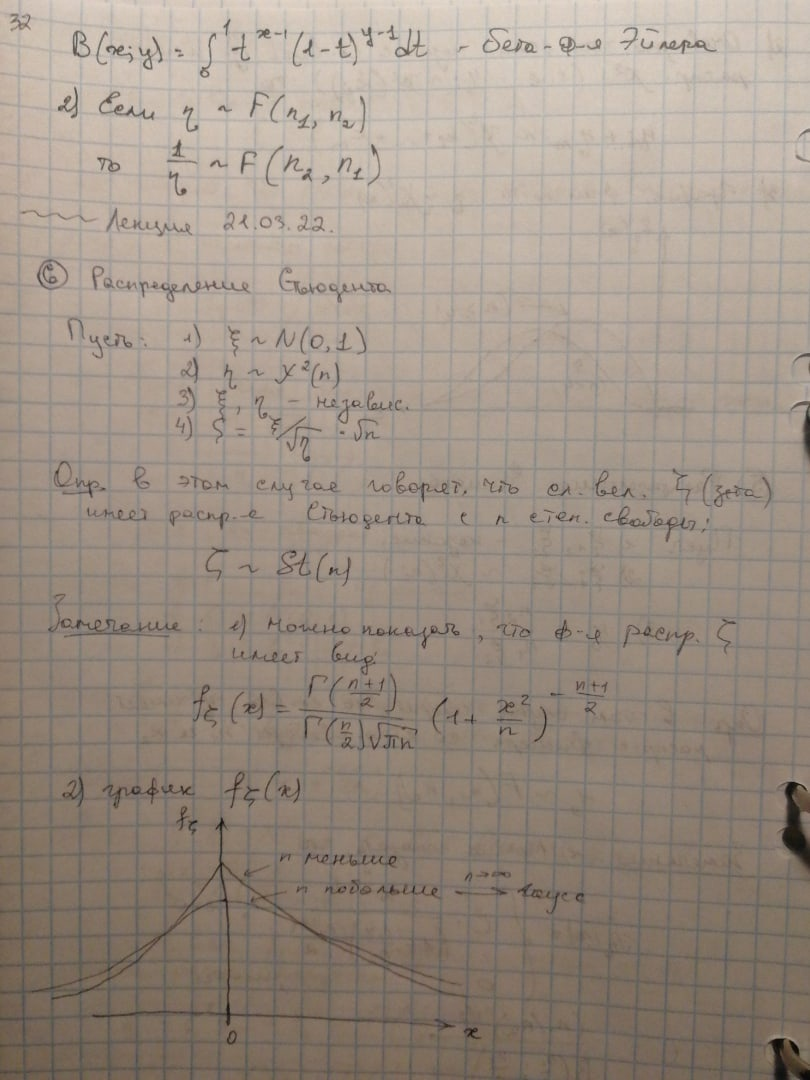
\includegraphics[scale=1.6]{1}}
\end{figure}

\begin{figure}[H]
	\center{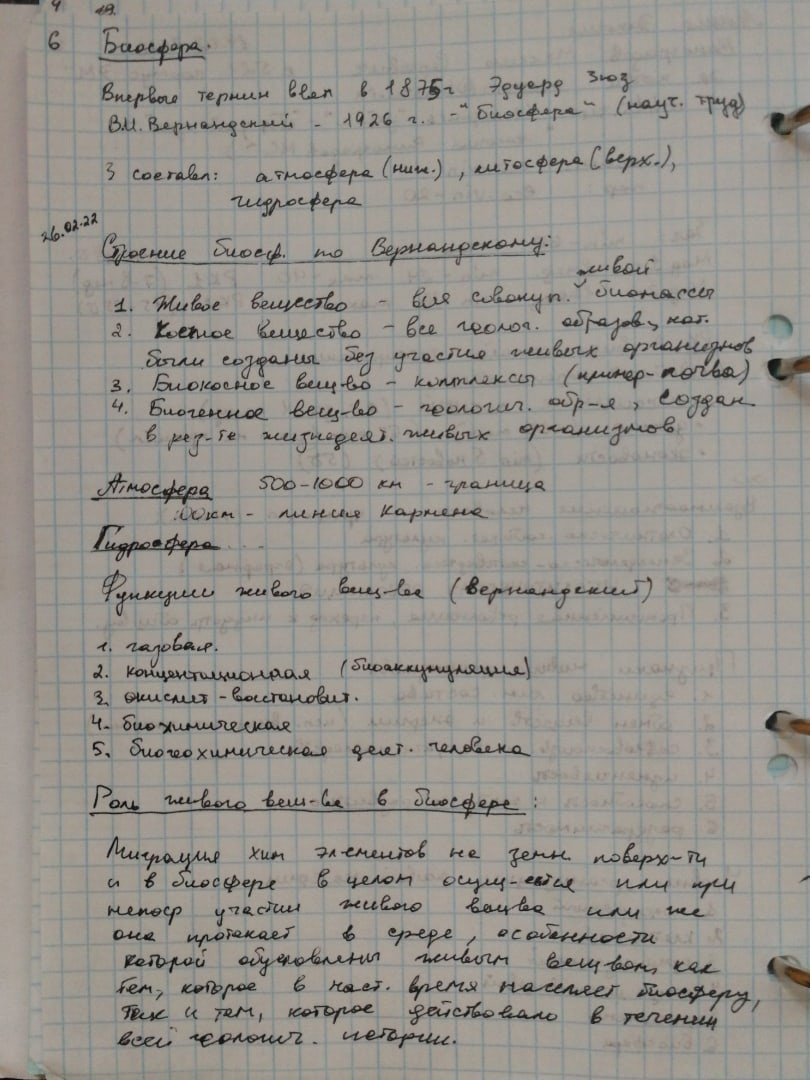
\includegraphics[scale=1.6]{2}}
\end{figure}